% **************************************************
% Document Class Definition
% **************************************************
\documentclass[%
	paper=A4,					% paper size --> A4 is default in Germany
	twoside=true,				% onesite or twoside printing
	openright,					% doublepage cleaning ends up right side
	parskip=full,				% spacing value / method for paragraphs
	chapterprefix=true,			% prefix for chapter marks
	11pt,						% font size
	headings=normal,			% size of headings
	bibliography=totoc,			% include bib in toc
	listof=totoc,				% include listof entries in toc
	titlepage=on,				% own page for each title page
	captions=tableabove,		% display table captions above the float env
	draft=false,				% value for draft version
]{scrreprt}%

% **************************************************
% Debug LaTeX Information
% **************************************************
%\listfiles

% **************************************************
% Information and Commands for Reuse
% **************************************************
\newcommand{\thesisTitle}{Bachelor Seminar}
\newcommand{\thesisName}{Marcel Fraas}
\newcommand{\thesisSubject}{Data Mining Frameworks}
\newcommand{\thesisDate}{4. Februar, 2017}
\newcommand{\thesisVersion}{Draft}

\newcommand{\thesisFirstReviewer}{Prof. Dr.-Ing. Stefan Jablonski}
\newcommand{\thesisFirstReviewerUniversity}{\protect{Universit{\"a}t Bayreuth}}
\newcommand{\thesisFirstReviewerDepartment}{Fakult{\"a}t Mathematik, Physik, Informatik}

\newcommand{\thesisSecondReviewer}{Dr. Stefan Sch{\"o}nig}
\newcommand{\thesisSecondReviewerUniversity}{\protect{Universit{\"a}t Bayreuth}}
\newcommand{\thesisSecondReviewerDepartment}{Fakult{\"a}t Mathematik, Physik, Informatik}

\newcommand{\thesisFirstSupervisor}{Stefan Sch{\"o}nig}
\newcommand{\thesisSecondSupervisor}{Lars Ackermann}

\newcommand{\thesisUniversity}{\protect{Universit{\"a}t Bayreuth}}
\newcommand{\thesisUniversityDepartment}{Fakult{\"a}t Mathematik, Physik, Informatik}
\newcommand{\thesisUniversityInstitute}{Institut f{\"u}r Informatik}
\newcommand{\thesisUniversityGroup}{Lehrstuhl f{\"u}r Angewandte Informatik IV}
\newcommand{\thesisUniversityCity}{Bayreuth}
\newcommand{\thesisUniversityStreetAddress}{Universit{\"a}tsstrasse 30}
\newcommand{\thesisUniversityPostalCode}{95447}

% **************************************************
% Load and Configure Packages
% **************************************************
\usepackage[utf8]{inputenc}		% defines file's character encoding
\usepackage[german]{babel} % babel system, adjust the language of the content
\usepackage[					% clean thesis style
	figuresep=colon,%
	sansserif=false,%
	hangfigurecaption=false,%
	hangsection=true,%
	hangsubsection=true,%
	colorize=full,%
	colortheme=bluemagenta,%
	bibsys=bibtex,%
	bibfile=bib-refs,%
	bibstyle=alphabetic,%
]{cleanthesis}

\hypersetup{					% setup the hyperref-package options
	pdftitle={\thesisTitle},	% 	- title (PDF meta)
	pdfsubject={\thesisSubject},% 	- subject (PDF meta)
	pdfauthor={\thesisName},	% 	- author (PDF meta)
	plainpages=false,			% 	-
	colorlinks=false,			% 	- colorize links?
	pdfborder={0 0 0},			% 	-
	breaklinks=true,			% 	- allow line break inside links
	bookmarksnumbered=true,		%
	bookmarksopen=true			%
}

% **************************************************
% Document CONTENT
% **************************************************
\begin{document}

% --------------------------
% rename document parts
% --------------------------
\renewcaptionname{ngerman}{\figurename}{Abb.}
\renewcaptionname{ngerman}{\tablename}{Tab.}
%\renewcaptionname{english}{\figurename}{Fig.}
%\renewcaptionname{english}{\tablename}{Tab.}

% --------------------------
% Front matter
% --------------------------
\pagenumbering{roman}			% roman page numbing (invisible for empty page style)
\pagestyle{empty}				% no header or footers
% !TEX root = ../Seminararbeit-Data_Mining_Frameworks.tex
%
% ------------------------------------  --> cover title page
\begin{titlepage}
	\pdfbookmark[0]{Cover}{Cover}
	
\includegraphics[width=10cm]{gfx/AI4.png} \\[2mm]
		\flushright
	\vfill
	{\LARGE\thesisTitle \par}
	\rule[5pt]{\textwidth}{.4pt} \par
	{\Large\thesisName}
	\vfill
	\textit{\large\thesisDate} \\
	Version: \thesisVersion
\end{titlepage}


% ------------------------------------  --> main title page
\begin{titlepage}
	\pdfbookmark[0]{Titlepage}{Titlepage}
	\tgherosfont
	\centering

	{\Large \thesisUniversity} \\[4mm]
	\textsf{\thesisUniversityDepartment} \\
	\textsf{\thesisUniversityInstitute} \\
	\textsf{\thesisUniversityGroup} \\

	\vfill
	{\large \thesisSubject} \\[5mm]
	{\LARGE \color{ctcolortitle}\textbf{\thesisTitle} \\[10mm]}
	{\Large \thesisName} \\

	\vfill
	\begin{minipage}[t]{.27\textwidth}
		\raggedleft
		\textit{1. Reviewer}
	\end{minipage}
	\hspace*{15pt}
	\begin{minipage}[t]{.65\textwidth}
		{\Large \thesisFirstReviewer} \\
	  	{\small \thesisFirstReviewerDepartment} \\[-1mm]
		{\small \thesisFirstReviewerUniversity}
	\end{minipage} \\[5mm]
	\begin{minipage}[t]{.27\textwidth}
		\raggedleft
		\textit{2. Reviewer}
	\end{minipage}
	\hspace*{15pt}
	\begin{minipage}[t]{.65\textwidth}
		{\Large \thesisSecondReviewer} \\
	  	{\small \thesisSecondReviewerDepartment} \\[-1mm]
		{\small \thesisSecondReviewerUniversity}
	\end{minipage} \\[10mm]
	\begin{minipage}[t]{.27\textwidth}
		\raggedleft
		\textit{Supervisors}
	\end{minipage}
	\hspace*{15pt}
	\begin{minipage}[t]{.65\textwidth}
		\thesisFirstSupervisor\ and \thesisSecondSupervisor
	\end{minipage} \\[10mm]

	\thesisDate \\

\end{titlepage}


% ------------------------------------  --> lower title back for single page layout
\hfill
\vfill
{
	\small
	\textbf{\thesisName} \\
	\textit{\thesisTitle} \\
	\thesisSubject, \thesisDate \\
	Reviewers: \thesisFirstReviewer\ and \thesisSecondReviewer \\
	Supervisors: \thesisFirstSupervisor\ and \thesisSecondSupervisor \\[1.5em]
	\textbf{\thesisUniversity} \\
	\textit{\thesisUniversityGroup} \\
	\thesisUniversityInstitute \\
	\thesisUniversityDepartment \\
	\thesisUniversityStreetAddress \\
	\thesisUniversityPostalCode\ \thesisUniversityCity\\ Germany
}
		% INCLUDE: all titlepages
\cleardoublepage

\pagestyle{plain}				% display just page numbers
%% !TEX root = ../Seminararbeit-Data_Mining_Frameworks.tex
%
\pdfbookmark[0]{Abstract}{Abstract}
\chapter*{Abstract}
\label{sec:abstract}
\vspace*{-10mm}

\blindtext

\vspace*{20mm}

{\usekomafont{chapter}Abstract (different language)}\label{sec:abstract-diff} \\

\blindtext
		% INCLUDE: the abstracts (english and german)
\cleardoublepage
%
\cleardoublepage
%
\setcounter{tocdepth}{2}		% define depth of toc
\tableofcontents				% display table of contents
\cleardoublepage

% --------------------------
% Body matter
% --------------------------
\pagenumbering{arabic}			% arabic page numbering
\setcounter{page}{1}			% set page counter
\pagestyle{maincontentstyle} 	% fancy header and footer

% !TEX root = ../Seminararbeit-Data_Mining_Frameworks.tex
%


% =============================================================================
%
% Einleitung: Grundlagen zu Data Mining
%
% =============================================================================
\chapter{Data Mining Grundlagen}
\label{sec:intro}

\cleanchapterquote{Information is not knowledge.}{Albert Einstein}{(Theoretischer Physiker)}

%\Blindtext[2][2]
Der Begriff Data Mining bezeichnet zunächst einmal das Sammeln, Verarbeiten und
Analysieren von Daten und den damit verbundenen Informationsgewinn. Da
allerdings in der echten Welt eine große Bandbreite an Anwendungen und
Problemfeldern existiert, versteht man unter dem „minen von Daten“ ein sehr
weit gefächertes Feld an Methoden zur Datenverarbeitung. \\
\\
Data Mining hat in unserem Alltag längst Einzug gefunden, meistens bemerken wir
dies jedoch gar nicht. Nutzen wir beim Einkaufen beispielsweise eine
Bonuspunkte-Karte, sind in sozialen Medien aktiv oder stehen auf dem Weg zur
Arbeit im Stau, generieren wir eine Unmenge an Daten. Diese werden von
Unternehmen gesammelt und anschließend ausgewertet. Innerhalb dieser Ansammlung
an Datensätzen finden sich Informationen über unsere Gewohnheiten, unsere
Interessen und über unser Verhalten. \\
Data Mining hilft uns, eben jene Informationen interpretierbar zu machen und
somit besser zu verstehen, wie Menschen mit ihrer Umwelt interagieren. \\
\\
Gleichzeitig muss man allerdings auch den Aspekt des Datenschutzes beachten.
Reicht das Sammeln von Daten zu weit in die Privatsphäre eines einzelnen,
kann dies schnell zum Missbrauch dieser Informationen führen. \\
\\
Dass das Thema Data Mining kontrovers ist zeigt auch der Artikel „How
Companies Learn Your Secrets“ aus dem New York Times Magazine. \cite{NYT:12} Hier wollte
eine amerikanische Supermarktkette das Kaufverhalten ihrer Kunden untersuchen.
Um dies zu bewerkstelligen, wurde den Kunden zunächst eine Identifikationsnummer
zugewiesen, sowie Namen, Kreditkarteninformationen und Email-Adresse
gespeichert. Unter Einbezug weiterer externer Datenquellen zur Demografie
konnten einige interessante Beobachtungen gemacht werden. So konnte die
Supermarktkette beispielsweise die Schwangerschaft von Frauen anhand der
Einkäufe erkennen und hat im Zuge dessen festgestellt, dass schwangere Frauen
im zweiten Trimester ihrer Schwangerschaft vermehrt geruchlose Lotionen kaufen.
Außerdem werden innerhalb der ersten 20 Wochen der Schwangerschaft häufiger
Zusatzstoffe wie Kalzium, Magnesium und Zink erworben. Nähert sich der Tag der
Entbindung, werden zunehmend geruchlose Seife und extra große Wattepads in
Verbindung mit Desinfektionsmittel und Waschlappen gekauft. \\
Mit diesen Informationen war es möglich, einen sog. „pregnancy prediction score“
zu errechnen, welcher dazu genutzt wurde, gezielt Werbung in Form von Gutscheinen
zu bestimmten Zeiten der Schwangerschaft zu verschicken. \\
Der Artikel beschreibt einen Vorfall, bei dem ein wütender Mann in eine der
Filialen der Supermarktkette kam und sich beschwerte, dass seine Tochter
Gutscheine für Babykleidung und Krippen bekam. Der Mann wolle nicht, dass seine
Tochter von der Supermarktkette dazu ermutigt werde, schwanger zu werden. Als
der Manager der Filiale später bei dem Vater anrief, um sich zu entschuldigen,
wurde ihm von diesem mitgeteilt, dass die Tochter tatsächlich schwanger sei, was der Vater
jedoch zum Zeitpunkt seiner Beschwerde nicht wusste. \\
\\
Dieses Beispiel zeigt, dass es wichtig ist, präzise abzuwägen, wie genau eine
Analyse der Daten sein sollte. \\
 % INCLUDE: introduction
% !TEX root = ../Seminararbeit-Data_Mining_Frameworks.tex
%


% =============================================================================
%
% Der Data Mining Prozess
%
% =============================================================================
\chapter{Der Data Mining Prozess}
\label{sec:process}

Der Prozess des Data Minings lässt sich grundsätzlich durch die folgenden Phasen
beschreiben:
\begin{enumerate}
\item Sammeln von Daten: \\
Für das Sammeln von Daten ist unter Umständen spezielle Hardware, bspw.
Sensoren, händische Arbeit wie das Sammeln von Umfragebögen oder Software in
Form einer Webanwendung mit auszufüllenden Formularfeldern, notwendig. Auch wenn
diese Phase sehr Anwendungsspezifisch ist und oft vom Daten-Analysten nicht
beeinflusst werden kann, ist sie ausschlaggebend für das Ergebnis des Data
Mining Prozesses.
\item Bereinigen der Daten: \\
Oftmals sind die gesammelten Rohdaten aufgrund des Dateiformats oder einer
fehlenden Struktur nicht direkt verarbeitbar. Deshalb ist es wichtig, die Daten
in ein Format zu bringen, welches von Data Mining Algorithmen gelesen werden
kann.
\item Analyse der Daten: \\
Der letzte Schritt ist die Daten analytisch zu verarbeiten und Methoden zu
entwickeln, um diese nutzbar zu machen. Dies geschieht durch das Anwenden von
bestimmten Data Mining Algorithmen, welche für die jeweilige Aufgabenstellung
angepasst werden müssen.
\end{enumerate}
Um einen Standard für einen solchen Data Mining Vorgang zu etablieren, haben
einige große Unternehmen wie Automobilhersteller Daimler-Benz, Versicherungs
Provider OHRA, Hard- und Software Hersteller NCR Corp. und Statistik-Software
Hersteller SPSS Inc. den „CRoss-Industry Standard Process for Data Mining“
(kurz: CRISP-DM) definiert.

\pagebreak

\section{CRISP-DM}
\label{sec:process:crispdm}

\begin{figure}[htb]
	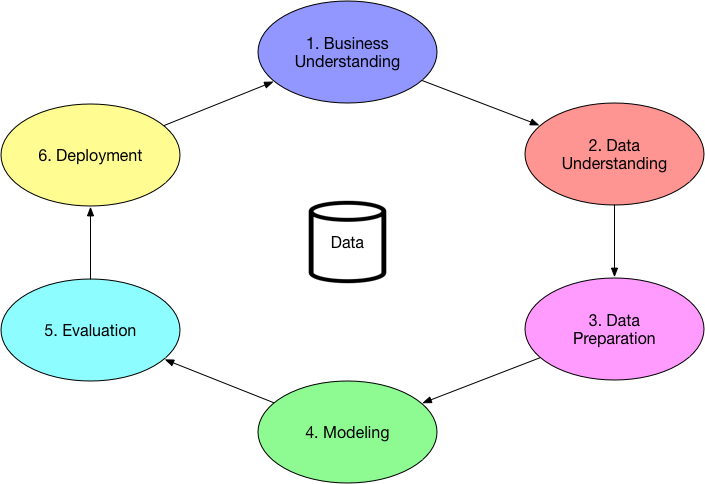
\includegraphics[width=\textwidth]{gfx/CRISP-DM_Model.png}
	\caption{Konzeptionelles CRISP-DM Modell}
	\label{fig:process:crispdm}
\end{figure}

\subsection{Business Understanding}
\label{sec:process:crispdm:bu}

Im ersten Schritt des CRISP-DM Prozesses, dem sog. Business- (oder auch Organizational-) Understanding,
ist es zunächst wichtig festzulegen was man mit dem Minen von Daten erreichen
möchte bzw. welche Informationen von Interesse sind. Hier findet auch eine oft
zitierte Textstelle aus Alice im Wunderland Anwendung:
\begin{quotation}
  >>Willst du mir wohl sagen, wenn ich bitten darf, welchen Weg ich hier nehmen muß?<< \\
  >>Das hängt zum guten Teil davon ab, wohin du gehen willst,<< sagte die Katze. \\
  >>Es kommt mir nicht darauf an, wohin –<< sagte Alice. \\
  >>Dann kommt es auch nicht darauf an, welchen Weg du nimmst,<< sagte die Katze. \\
  >>– wenn ich nur irgendwo hinkomme,<< fügte Alice als Erklärung hinzu. \\
  >>O, das wirst du ganz gewiß,« sagte die Katze, »wenn du nur lange genug gehest.<<
\end{quotation}
Konkret bedeutet das, dass es keine Rolle spielt wie lange man Daten Mined, wenn
man nicht festgelegt hat welche Informationen man gerne hätte. Es müssen also
zunächst Fragen festgelegt werden, welche durch das Data Mining beantwortet
werden sollen. Beispielsweise möchte man gerne wissen warum sich Kunden so sehr
beschweren, wie man die Profit-Spanne seiner Produkte vergrößert oder wie man
Fehler bei der Herstellung antizipieren kann.

\subsection{Data Understanding}
\label{sec:process:crispdm:du}



\subsection{Data Preparation}
\label{sec:process:crispdm:dp}

\subsection{Modeling}
\label{sec:process:crispdm:mod}

\subsection{Evaluation}
\label{sec:process:crispdm:eval}

\subsection{Deployment}
\label{sec:process:crispdm:depl}

\section{Alternativen}
\label{sec:alt}

% !TEX root = ../Seminararbeit-Data_Mining_Frameworks.tex
%
\chapter{Related Work}
\label{sec:related}

\cleanchapterquote{A picture is worth a thousand words. An interface is worth a thousand pictures.}{Ben Shneiderman}{(Professor for Computer Science)}

\Blindtext[2][1]

\section{Related Work Section 1}
\label{sec:related:sec1}

\Blindtext[2][2]

\section{Related Work Section 2}
\label{sec:related:sec2}

\Blindtext[3][2]

\section{Related Work Section 3}
\label{sec:related:sec3}

\Blindtext[4][2]

\section{Conclusion}
\label{sec:related:conclusion}

\Blindtext[2][1]
 % INCLUDE: related work
% !TEX root = ../Seminararbeit-Data_Mining_Frameworks.tex
%
\chapter{System}
\label{sec:system}

\cleanchapterquote{Innovation distinguishes between a leader and a follower.}{Steve Jobs}{(CEO Apple Inc.)}

\Blindtext[2][1]

\section{System Section 1}
\label{sec:system:sec1}

\Blindtext[1][2]

\begin{figure}[htb]
	
\includegraphics[width=\textwidth]{gfx/Clean-Thesis-Figure}
	\caption{Figure example: \textit{(a)} example part one, \textit{(c)} example part two; \textit{(c)} example part three}
	\label{fig:system:example1}
\end{figure}

\Blindtext[1][2]

\section{System Section 2}
\label{sec:system:sec2}

\Blindtext[1][2]

\begin{figure}[htb]
	
\includegraphics[width=\textwidth]{gfx/Clean-Thesis-Figure}
	\caption{Another Figure example: \textit{(a)} example part one, \textit{(c)} example part two; \textit{(c)} example part three}
	\label{fig:system:example2}
\end{figure}

\Blindtext[2][2]

\section{System Section 3}
\label{sec:system:sec3}

\Blindtext[4][2]

\section{Conclusion}
\label{sec:system:conclusion}

\Blindtext[2][1]
	% INCLUDE: system
% !TEX root = ../Seminararbeit-Data_Mining_Frameworks.tex
%
\chapter{Concepts}
\label{sec:concepts}

\cleanchapterquote{Users do not care about what is inside the box, as long as the box does what they need done.}{Jef Raskin}{about Human Computer Interfaces}

\Blindtext[2][1]

\section{Concepts Section 1}
\label{sec:concepts:sec1}

\Blindtext[2][2]

\section{Concepts Section 2}
\label{sec:concepts:sec2}

\Blindtext[3][2]

\section{Concepts Section 3}
\label{sec:concepts:sec3}

\Blindtext[4][2]

\section{Conclusion}
\label{sec:concepts:conclusion}

\Blindtext[2][1]
 % INCLUDE: concepts
% !TEX root = ../Seminararbeit-Data_Mining_Frameworks.tex
%
\chapter{Conclusion}
\label{sec:conclusion}

\Blindtext[2][1]

\section{System Section 1}
\label{sec:conclusion:sec1}

\Blindtext[2][2]

\section{System Section 2}
\label{sec:conclusion:sec2}

\Blindtext[3][2]

\section{Future Work}
\label{sec:conclusion:future}

\Blindtext[2][2]
 % INCLUDE: conclusion
\cleardoublepage

% --------------------------
% Back matter
% --------------------------
{%
\setstretch{1.1}
\renewcommand{\bibfont}{\normalfont\small}
\setlength{\biblabelsep}{0pt}
\setlength{\bibitemsep}{0.5\baselineskip plus 0.5\baselineskip}
\printbibliography[nottype=online]
\printbibliography[heading=subbibliography,title={Websites},type=online,prefixnumbers={@}]
}
\cleardoublepage

\listoffigures
\cleardoublepage

\listoftables
\cleardoublepage

% !TEX root = ../Seminararbeit-Data_Mining_Frameworks.tex
%
%************************************************
% Declaration
%************************************************
\pdfbookmark[0]{Declaration}{Declaration}
\chapter*{Declaration}
\label{sec:declaration}
\thispagestyle{empty}

You can put your declaration here, to declare that you have completed your work solely and only with the help of the references you mentioned.

\bigskip

\noindent\textit{\thesisUniversityCity, \thesisDate}

\smallskip

\begin{flushright}
	\begin{minipage}{5cm}
		\rule{\textwidth}{1pt}
		\centering\thesisName
	\end{minipage}
\end{flushright}

%*****************************************
%*****************************************

\clearpage
\newpage
\mbox{}

% **************************************************
% End of Document CONTENT
% **************************************************
\end{document}
